\documentclass[10 pt,usenames,dvipsnames, oneside]{article}
\usepackage{../../../modelo-ensino-medio}



\begin{document}

\begin{center}
  \begin{minipage}[l]{3cm}

\includegraphics[width=2cm]{logo}    
\end{minipage}\hfill
\begin{minipage}[r]{.8\textwidth}
 {\Large \scshape Atividade: Fases da Lua}  
\end{minipage}
\end{center}
\vspace{.2cm}

\ifdefined\prof
%Habilidades da BNCC
% \begin{objetivos}
% \item 
% \end{objetivos}

%Caixa do Para o Professor
\begin{goals}
%Objetivos específicos
\begin{enumerate}
\item Realizar a modelagem de situações problema por meio do
recurso a fenômenos periódicos;
\item Reconhecer as transformações geométricas associadas a
parâmetros aplicados às expressões analíticas das funções
seno e cosseno no esboço do seu gráfico.
\item Fazer previsões baseado em modelagem de fenômenos
periódicos;
\end{enumerate}

\tcblower

%Orientações e sugestões
\begin{itemize}
\item Professor, trabalhe com a representação decimal da
porcentagem para que o gráfico não fique muito \textbf{esticado
verticalmente}.
\item Usando os valores máximo $(1)$ e mínimo $(0)$, conclua que a
amplitude é $0{,}5$ e, portanto, $a=d=0{,}5$
\item Usando que o período é $30$, conclua que $b=\dfrac{2\pi}{30}$
\end{itemize}
\end{goals}

\bigskip
\begin{center}
{\large \scshape Atividade}
\end{center}
\fi

Plote no GeoGebra os pontos $(t,y)$, onde $t$ é o dia e $y$ é o percentual de visibilidade da lua no dia $t$. Faça isso para todos os dias de junho.

\begin{figure}[H]
\centering

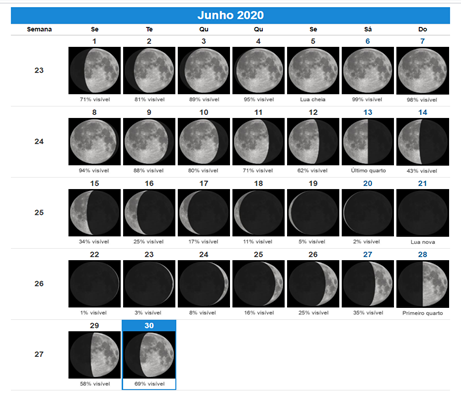
\includegraphics[width=.6\linewidth]{trigonometricas115}
\caption{Fonte: \href{https://www.calendario-365.com.br/calend\%C3\%A1rio-lunar/2020/junho.html}{Calendário 365}}
\label{}
\end{figure}

Encontre uma função trigonométrica da forma $y = a\cdot\sen(bt+c) +d$ que melhor se aproxima dos pontos traçados. Use-a para prever a fase da lua nos dias 01 a 14 de julho. Compare o resultado obtido por você com o que consta no site \url{https://www.calendario-365.com.br/calendário-lunar/2020/julho.html}

\begin{figure}[H]
\centering

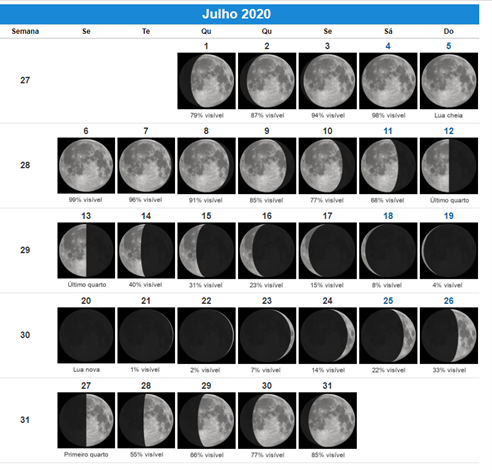
\includegraphics[width=.6\linewidth]{trigonometricas116}
\end{figure}

\ifdefined\prof
\begin{solucao}

\begin{itemize}
\item $a=0{,}5; b=\dfrac{2\pi}{30};c=0{,}3; d=0{,}5$
\item Dia 1 de julho, $74\%$; $(f(31)=0{,}74)$
\item Dia 14 de julho, $45\%$. $(f(44)=0{,}45)$
\end{itemize}
\end{solucao}
\fi

\end{document}